\documentclass[a4paper]{book}
\usepackage{a4wide}
\usepackage{makeidx}
\usepackage{graphicx}
\usepackage{multicol}
\usepackage{float}
\usepackage{listings}
\usepackage{color}
\usepackage{textcomp}
\usepackage{alltt}
\usepackage{times}
\usepackage{ifpdf}
\ifpdf
\usepackage[pdftex,
            pagebackref=true,
            colorlinks=true,
            linkcolor=blue,
            unicode
           ]{hyperref}
\else
\usepackage[ps2pdf,
            pagebackref=true,
            colorlinks=true,
            linkcolor=blue,
            unicode
           ]{hyperref}
\usepackage{pspicture}
\fi
\usepackage[utf8]{inputenc}
\usepackage{doxygen}
\lstset{language=C++,inputencoding=utf8,basicstyle=\footnotesize,breaklines=true,breakatwhitespace=true,tabsize=8,numbers=left }
\makeindex
\setcounter{tocdepth}{3}
\renewcommand{\footrulewidth}{0.4pt}
\begin{document}
\hypersetup{pageanchor=false}
\begin{titlepage}
\vspace*{7cm}
\begin{center}
{\Large mypopen\_\-mypclose \\[1ex]\large 2.0.0 }\\
\vspace*{1cm}
{\large Generated by Doxygen 1.6.1}\\
\vspace*{0.5cm}
{\small Sun Apr 17 09:50:11 2016}\\
\end{center}
\end{titlepage}
\clearemptydoublepage
\pagenumbering{roman}
\tableofcontents
\clearemptydoublepage
\pagenumbering{arabic}
\hypersetup{pageanchor=true}
\chapter{File Index}
\section{File List}
Here is a list of all files with brief descriptions:\begin{DoxyCompactList}
\item\contentsline{section}{\hyperlink{mypopen_8c}{mypopen.c} }{\pageref{mypopen_8c}}{}
\item\contentsline{section}{\hyperlink{mypopen_8h}{mypopen.h} }{\pageref{mypopen_8h}}{}
\end{DoxyCompactList}

\chapter{File Documentation}
\hypertarget{mypopen_8c}{
\section{mypopen.c File Reference}
\label{mypopen_8c}\index{mypopen.c@{mypopen.c}}
}
{\ttfamily \#include \char`\"{}mypopen.h\char`\"{}}\par
Include dependency graph for mypopen.c:\nopagebreak
\begin{figure}[H]
\begin{center}
\leavevmode
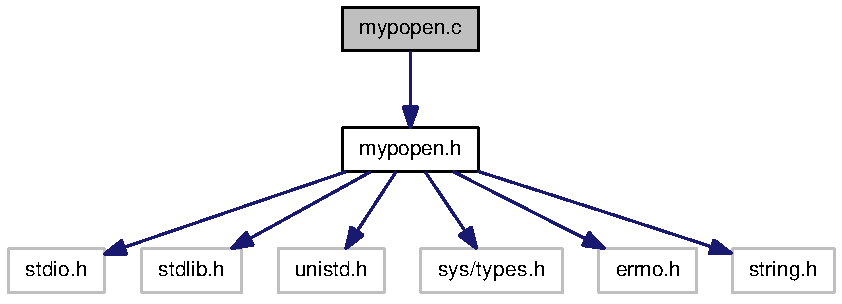
\includegraphics[width=260pt]{mypopen_8c__incl}
\end{center}
\end{figure}
\subsection*{Functions}
\begin{DoxyCompactItemize}
\item 
FILE $\ast$ \hyperlink{mypopen_8c_ac47876a41dddae340e5afa64489dec86}{mypopen} (const char $\ast$command, const char $\ast$type)
\item 
int \hyperlink{mypopen_8c_ae75ec57d5d9b3ad79c5f5e48e5dcfd0d}{mypclose} (FILE $\ast$stream)
\item 
static void \hyperlink{mypopen_8c_a974c9687b94a06aadad2daab081db4ba}{childAction} (int fd\mbox{[}2\mbox{]}, int unused\_\-end, int used\_\-end, const char $\ast$command, int fileno)
\item 
static FILE $\ast$ \hyperlink{mypopen_8c_a1ee8542fc9a69bf1be706ed8c632ab69}{parentAction} (int fd\mbox{[}2\mbox{]}, int unused\_\-end, int used\_\-end, const char $\ast$type)
\end{DoxyCompactItemize}
\subsection*{Variables}
\begin{DoxyCompactItemize}
\item 
static FILE $\ast$ \hyperlink{mypopen_8c_aa065f30aa9f5f9a42132c82c787ee70b}{fp} = NULL
\item 
static pid\_\-t \hyperlink{mypopen_8c_a8aecc963beadbaa964f33e98502b0526}{childpid}
\end{DoxyCompactItemize}


\subsection{Detailed Description}
mypopen\_\-mypclose Beispiel 2

\begin{DoxyAuthor}{Author}
Karin Kalman $<$\href{mailto:karin.kalman@technikum-wien.at}{\tt karin.kalman@technikum-\/wien.at}$>$ 

Michael Mueller $<$\href{mailto:michael.mueller@technikum-wien.at}{\tt michael.mueller@technikum-\/wien.at}$>$ 

Gerhard Sabeditsch $<$\href{mailto:gerhard.sabeditsch@technikum-wien.at}{\tt gerhard.sabeditsch@technikum-\/wien.at}$>$ 
\end{DoxyAuthor}
\begin{DoxyDate}{Date}
2016/04/17
\end{DoxyDate}
\begin{DoxyVersion}{Version}

\end{DoxyVersion}
Revision}
2 

URL: \$HeadURL\$

Last Modified: Author}
Gerhard 

Definition in file \hyperlink{mypopen_8c_source}{mypopen.c}.

\subsection{Function Documentation}
\hypertarget{mypopen_8c_a974c9687b94a06aadad2daab081db4ba}{
\index{mypopen.c@{mypopen.c}!childAction@{childAction}}
\index{childAction@{childAction}!mypopen.c@{mypopen.c}}
\subsubsection[{childAction}]{\setlength{\rightskip}{0pt plus 5cm}static void childAction (int {\em fd}\mbox{[}2\mbox{]}, \/  int {\em unused\_\-end}, \/  int {\em used\_\-end}, \/  const char $\ast$ {\em command}, \/  int {\em fileno})\hspace{0.3cm}{\ttfamily  \mbox{[}static\mbox{]}}}}
\label{mypopen_8c_a974c9687b94a06aadad2daab081db4ba}
-\/-\/-\/-\/-\/-\/-\/-\/-\/-\/-\/-\/-\/-\/-\/-\/-\/-\/-\/-\/-\/-\/-\/-\/-\/-\/-\/-\/-\/-\/-\/-\/-\/-\/-\/-\/-\/-\/-\/-\/-\/-\/-\/-\/-\/-\/-\/-\/-\/-\/-\/-\/-\/-\/-\/-\/-\/-\/-\/-\/-\/-\/ help -\/ functions -\/-\/ static void childAction(int fd\mbox{[}2\mbox{]}, int unused\_\-end, int used\_\-end, const char $\ast$command) FUNCTION is only for the CHILD PROCESS: -\/this function link the used file descriptor with the parent process stdout -\/this function also close the unused file descriptor -\/this function executes the given command in a normal shell like popen 

Definition at line 182 of file mypopen.c.

Referenced by mypopen().\hypertarget{mypopen_8c_ae75ec57d5d9b3ad79c5f5e48e5dcfd0d}{
\index{mypopen.c@{mypopen.c}!mypclose@{mypclose}}
\index{mypclose@{mypclose}!mypopen.c@{mypopen.c}}
\subsubsection[{mypclose}]{\setlength{\rightskip}{0pt plus 5cm}int mypclose (FILE $\ast$ {\em stream})}}
\label{mypopen_8c_ae75ec57d5d9b3ad79c5f5e48e5dcfd0d}
-\/-\/-\/-\/-\/-\/-\/-\/-\/-\/-\/-\/-\/-\/-\/-\/-\/-\/-\/-\/-\/-\/-\/-\/-\/-\/-\/-\/-\/-\/-\/-\/-\/-\/-\/-\/-\/-\/-\/-\/-\/-\/-\/-\/-\/-\/-\/-\/-\/-\/-\/-\/-\/-\/-\/-\/-\/-\/-\/-\/-\/-\/ mypclose -\/function -\/-\/ 

Definition at line 110 of file mypopen.c.

References childpid, and fp.\hypertarget{mypopen_8c_ac47876a41dddae340e5afa64489dec86}{
\index{mypopen.c@{mypopen.c}!mypopen@{mypopen}}
\index{mypopen@{mypopen}!mypopen.c@{mypopen.c}}
\subsubsection[{mypopen}]{\setlength{\rightskip}{0pt plus 5cm}FILE$\ast$ mypopen (const char $\ast$ {\em command}, \/  const char $\ast$ {\em type})}}
\label{mypopen_8c_ac47876a41dddae340e5afa64489dec86}
-\/-\/-\/-\/-\/-\/-\/-\/-\/-\/-\/-\/-\/-\/-\/-\/-\/-\/-\/-\/-\/-\/-\/-\/-\/-\/-\/-\/-\/-\/-\/-\/-\/-\/-\/-\/-\/-\/-\/-\/-\/-\/-\/-\/-\/-\/-\/-\/-\/-\/-\/-\/-\/-\/-\/-\/-\/-\/-\/-\/-\/-\/ mypopen -\/function -\/-\/ 

Open new pipe
\begin{DoxyItemize}
\item return value fd\mbox{[}0\mbox{]} is for reading
\item return value fd\mbox{[}1\mbox{]} is for writing
\end{DoxyItemize}

if fork() is successful it return twice:
\begin{DoxyItemize}
\item in parent process the return value is the process id (PID) of the childprocess
\item in child process the return value is 0
\end{DoxyItemize}

Child process

Parent process 

Definition at line 33 of file mypopen.c.

References childAction(), childpid, fp, parentAction(), READ\_\-END, and WRITE\_\-END.

Here is the call graph for this function:\nopagebreak
\begin{figure}[H]
\begin{center}
\leavevmode
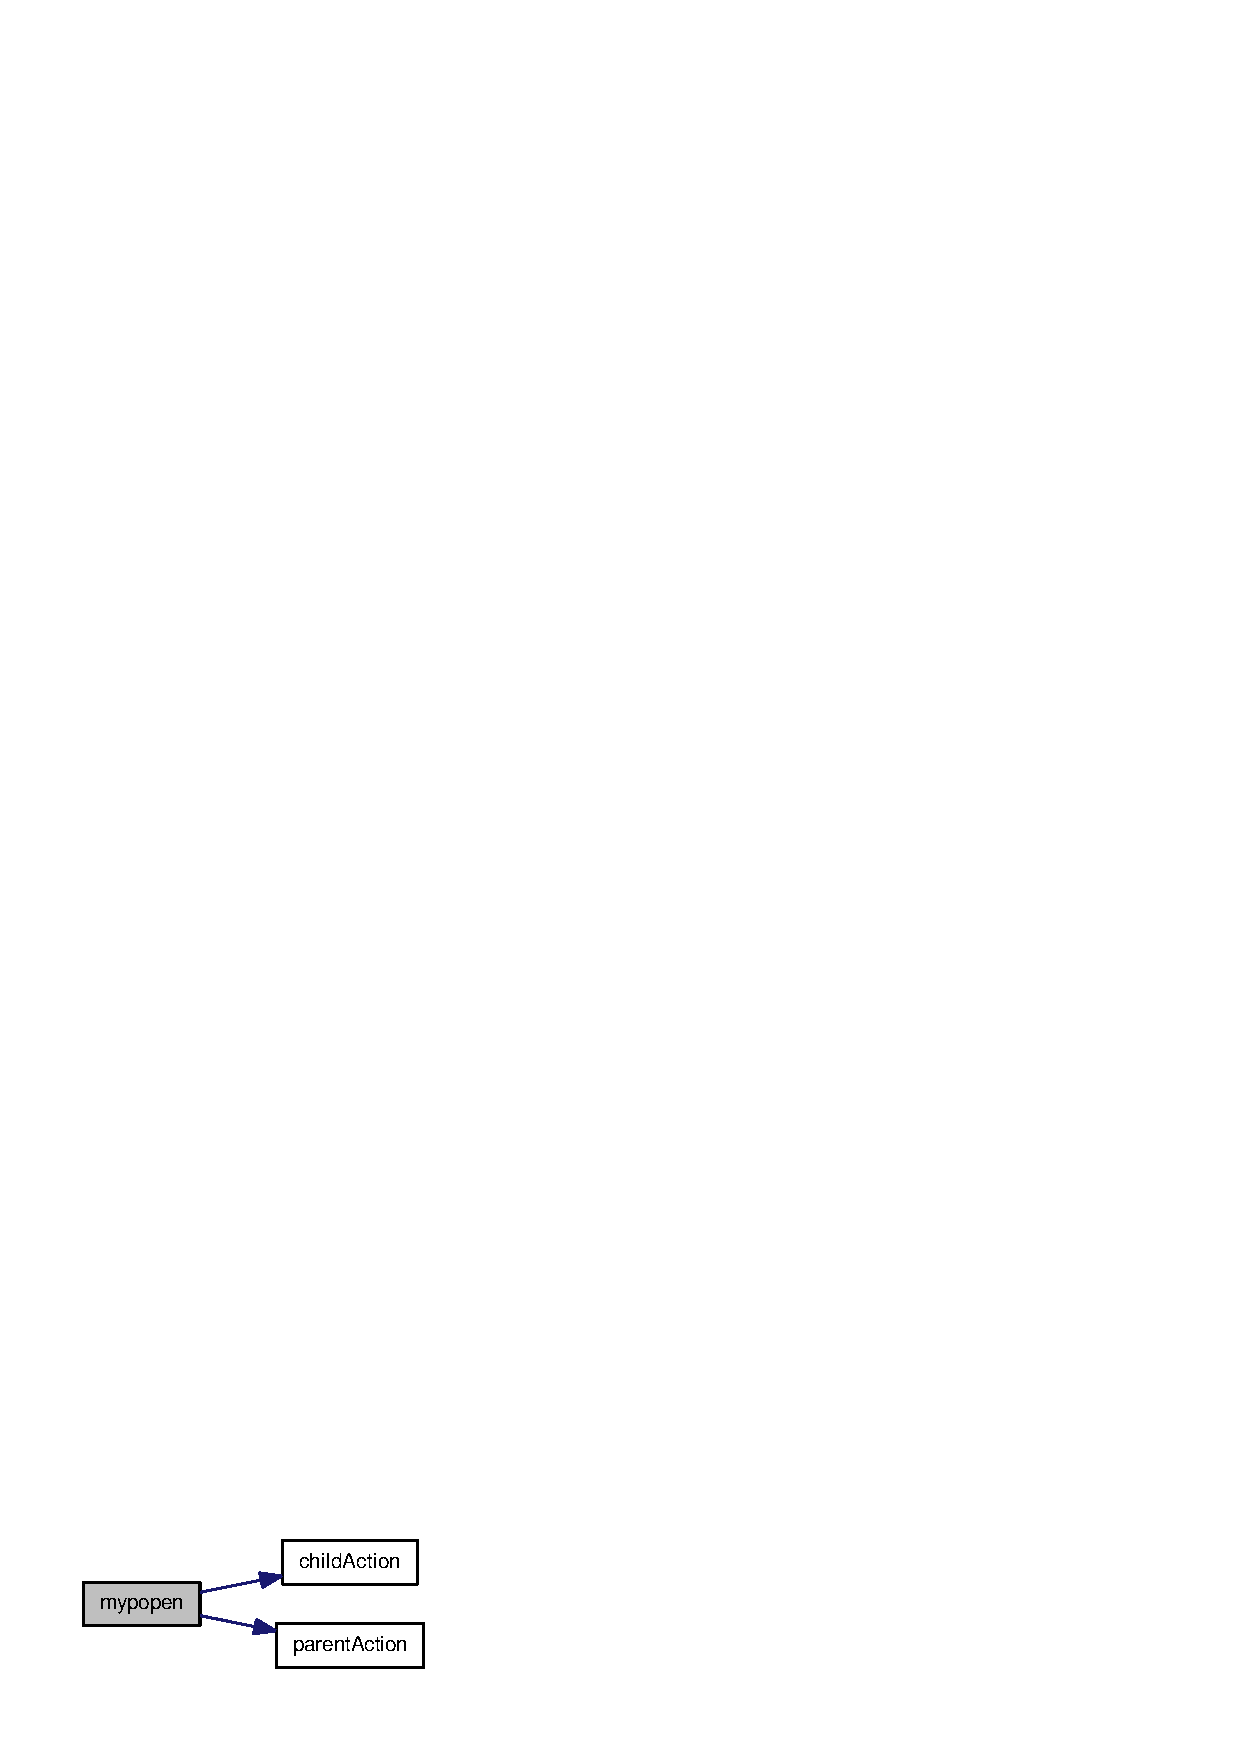
\includegraphics[width=104pt]{mypopen_8c_ac47876a41dddae340e5afa64489dec86_cgraph}
\end{center}
\end{figure}
\hypertarget{mypopen_8c_a1ee8542fc9a69bf1be706ed8c632ab69}{
\index{mypopen.c@{mypopen.c}!parentAction@{parentAction}}
\index{parentAction@{parentAction}!mypopen.c@{mypopen.c}}
\subsubsection[{parentAction}]{\setlength{\rightskip}{0pt plus 5cm}static FILE$\ast$ parentAction (int {\em fd}\mbox{[}2\mbox{]}, \/  int {\em unused\_\-end}, \/  int {\em used\_\-end}, \/  const char $\ast$ {\em type})\hspace{0.3cm}{\ttfamily  \mbox{[}static\mbox{]}}}}
\label{mypopen_8c_a1ee8542fc9a69bf1be706ed8c632ab69}
static FILE $\ast$ parentAction(int fd\mbox{[}2\mbox{]}, int unused\_\-end, int used\_\-end, const char $\ast$type) FUNCTION is only for the PARENT PROCESS: -\/this function link the used file descriptor with the parent process stin -\/this function also close the unused file descriptor -\/this function convert the used filedescriptor into a filepointer and returns the filepointer 

Definition at line 210 of file mypopen.c.

Referenced by mypopen().

\subsection{Variable Documentation}
\hypertarget{mypopen_8c_a8aecc963beadbaa964f33e98502b0526}{
\index{mypopen.c@{mypopen.c}!childpid@{childpid}}
\index{childpid@{childpid}!mypopen.c@{mypopen.c}}
\subsubsection[{childpid}]{\setlength{\rightskip}{0pt plus 5cm}pid\_\-t {\bf childpid}\hspace{0.3cm}{\ttfamily  \mbox{[}static\mbox{]}}}}
\label{mypopen_8c_a8aecc963beadbaa964f33e98502b0526}


Definition at line 28 of file mypopen.c.

Referenced by mypclose(), and mypopen().\hypertarget{mypopen_8c_aa065f30aa9f5f9a42132c82c787ee70b}{
\index{mypopen.c@{mypopen.c}!fp@{fp}}
\index{fp@{fp}!mypopen.c@{mypopen.c}}
\subsubsection[{fp}]{\setlength{\rightskip}{0pt plus 5cm}FILE$\ast$ {\bf fp} = NULL\hspace{0.3cm}{\ttfamily  \mbox{[}static\mbox{]}}}}
\label{mypopen_8c_aa065f30aa9f5f9a42132c82c787ee70b}
-\/-\/-\/-\/-\/-\/-\/-\/-\/-\/-\/-\/-\/-\/-\/-\/-\/-\/-\/-\/-\/-\/-\/-\/-\/-\/-\/-\/-\/-\/-\/-\/-\/-\/-\/-\/-\/-\/-\/-\/-\/-\/-\/-\/-\/-\/-\/-\/-\/-\/-\/-\/-\/-\/-\/-\/-\/-\/-\/-\/-\/-\/ includes -\/-\/ -\/-\/-\/-\/-\/-\/-\/-\/-\/-\/-\/-\/-\/-\/-\/-\/-\/-\/-\/-\/-\/-\/-\/-\/-\/-\/-\/-\/-\/-\/-\/-\/-\/-\/-\/-\/-\/-\/-\/-\/-\/-\/-\/-\/-\/-\/-\/-\/-\/-\/-\/-\/-\/-\/-\/-\/-\/-\/-\/-\/-\/-\/ global static variables -\/-\/ 

Definition at line 27 of file mypopen.c.

Referenced by mypclose(), and mypopen().
\hypertarget{mypopen_8h}{
\section{mypopen.h File Reference}
\label{mypopen_8h}\index{mypopen.h@{mypopen.h}}
}
{\ttfamily \#include $<$stdio.h$>$}\par
{\ttfamily \#include $<$stdlib.h$>$}\par
{\ttfamily \#include $<$unistd.h$>$}\par
{\ttfamily \#include $<$sys/types.h$>$}\par
{\ttfamily \#include $<$sys/wait.h$>$}\par
{\ttfamily \#include $<$errno.h$>$}\par
{\ttfamily \#include $<$string.h$>$}\par
Include dependency graph for mypopen.h:\nopagebreak
\begin{figure}[H]
\begin{center}
\leavevmode
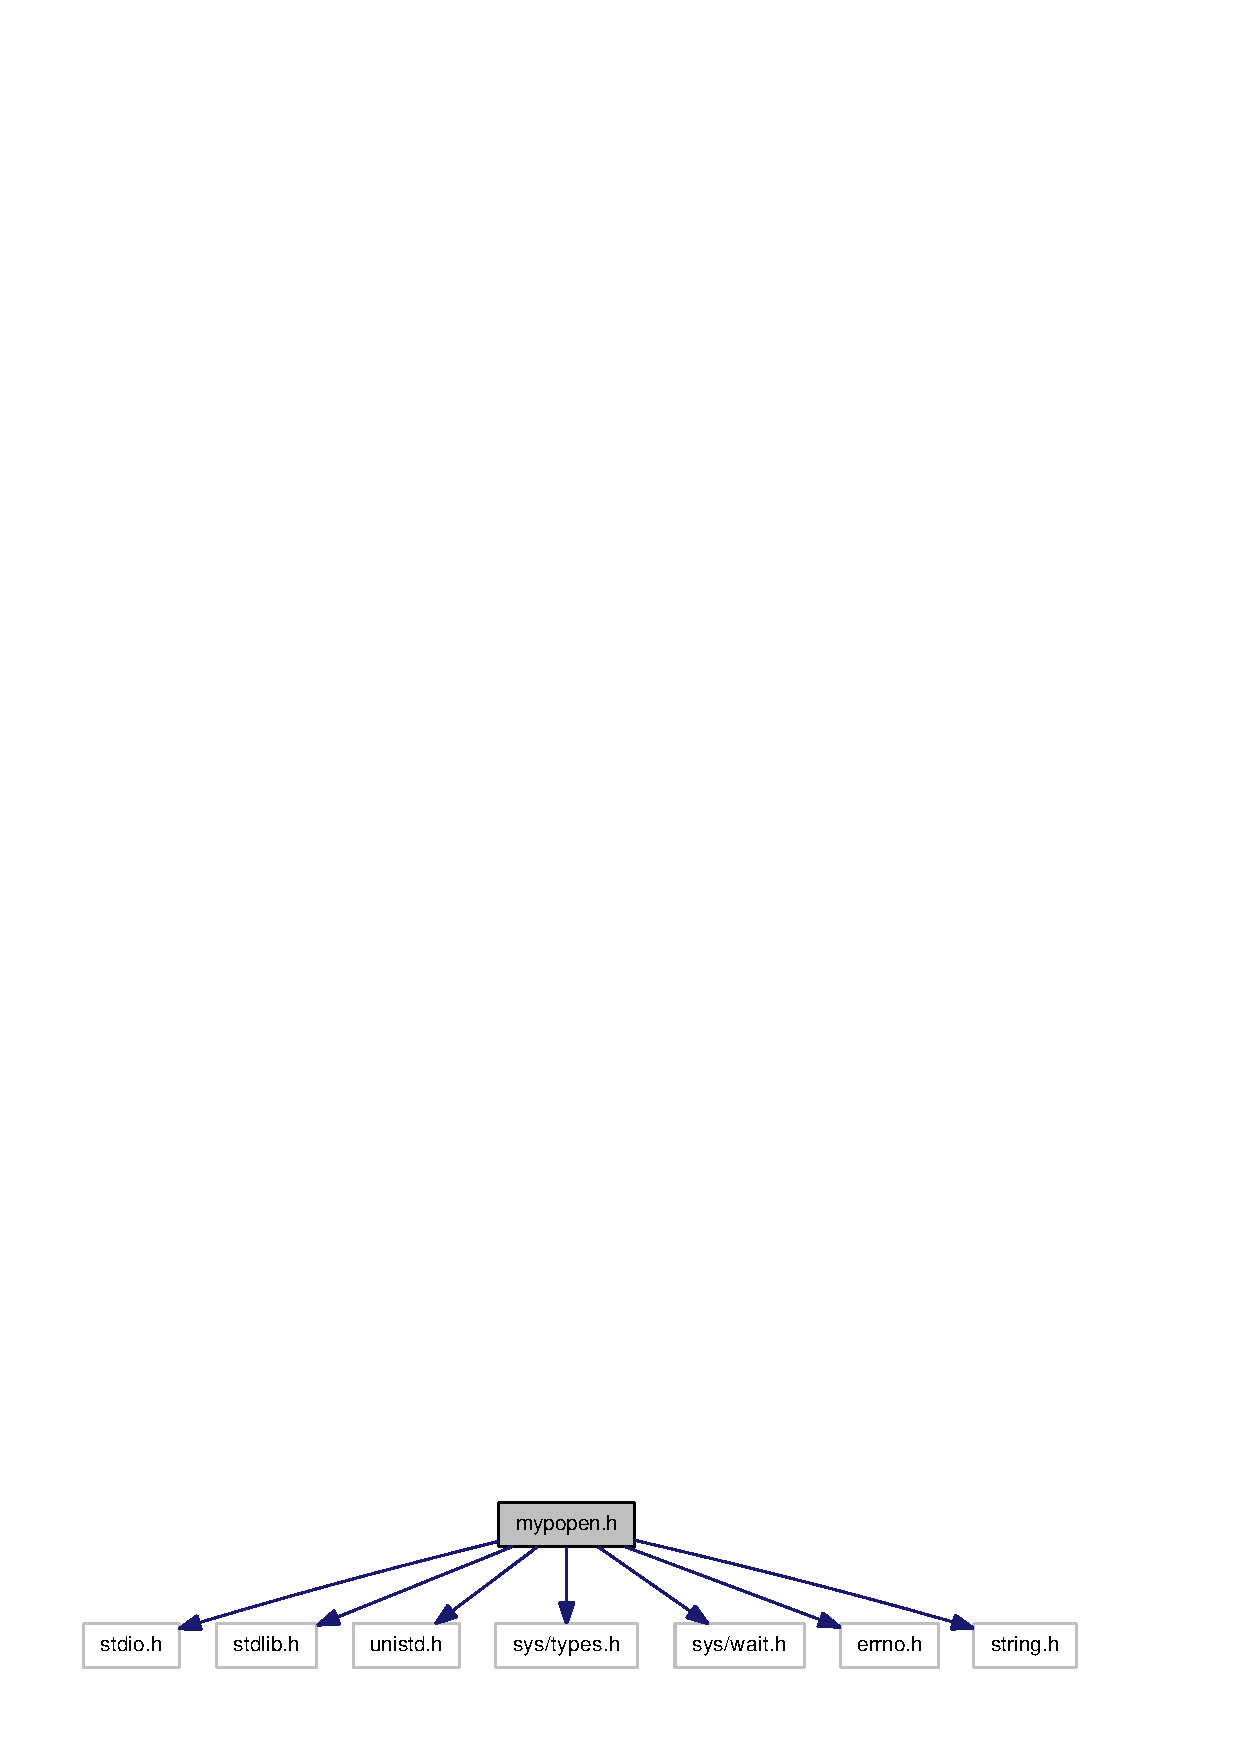
\includegraphics[width=260pt]{mypopen_8h__incl}
\end{center}
\end{figure}
This graph shows which files directly or indirectly include this file:\nopagebreak
\begin{figure}[H]
\begin{center}
\leavevmode
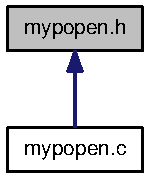
\includegraphics[width=54pt]{mypopen_8h__dep__incl}
\end{center}
\end{figure}
\subsection*{Defines}
\begin{DoxyCompactItemize}
\item 
\#define \hyperlink{mypopen_8h_a2469c53816dc077f9deefb187ffcabf3}{READ\_\-END}~0
\item 
\#define \hyperlink{mypopen_8h_a2efd706d915e621e5e18b3f0803c4ed2}{WRITE\_\-END}~1
\end{DoxyCompactItemize}
\subsection*{Functions}
\begin{DoxyCompactItemize}
\item 
FILE $\ast$ \hyperlink{mypopen_8h_ac47876a41dddae340e5afa64489dec86}{mypopen} (const char $\ast$command, const char $\ast$type)
\item 
int \hyperlink{mypopen_8h_ae75ec57d5d9b3ad79c5f5e48e5dcfd0d}{mypclose} (FILE $\ast$stream)
\item 
static void \hyperlink{mypopen_8h_a974c9687b94a06aadad2daab081db4ba}{childAction} (int fd\mbox{[}2\mbox{]}, int unused\_\-end, int used\_\-end, const char $\ast$command, int fileno)
\item 
static FILE $\ast$ \hyperlink{mypopen_8h_a1ee8542fc9a69bf1be706ed8c632ab69}{parentAction} (int fd\mbox{[}2\mbox{]}, int unused\_\-end, int used\_\-end, const char $\ast$type)
\end{DoxyCompactItemize}


\subsection{Detailed Description}
mypopen\_\-mypclose Beispiel 2

\begin{DoxyAuthor}{Author}
Karin Kalman $<$\href{mailto:karin.kalman@technikum-wien.at}{\tt karin.kalman@technikum-\/wien.at}$>$ 

Michael Mueller $<$\href{mailto:michael.mueller@technikum-wien.at}{\tt michael.mueller@technikum-\/wien.at}$>$ 

Gerhard Sabeditsch $<$\href{mailto:gerhard.sabeditsch@technikum-wien.at}{\tt gerhard.sabeditsch@technikum-\/wien.at}$>$ 
\end{DoxyAuthor}
\begin{DoxyDate}{Date}
2016/04/17
\end{DoxyDate}
\begin{DoxyVersion}{Version}

\end{DoxyVersion}
Revision}
1 

URL: \$HeadURL\$

Last Modified: Author}
Gerhard 

Definition in file \hyperlink{mypopen_8h_source}{mypopen.h}.

\subsection{Define Documentation}
\hypertarget{mypopen_8h_a2469c53816dc077f9deefb187ffcabf3}{
\index{mypopen.h@{mypopen.h}!READ\_\-END@{READ\_\-END}}
\index{READ\_\-END@{READ\_\-END}!mypopen.h@{mypopen.h}}
\subsubsection[{READ\_\-END}]{\setlength{\rightskip}{0pt plus 5cm}\#define READ\_\-END~0}}
\label{mypopen_8h_a2469c53816dc077f9deefb187ffcabf3}


Definition at line 39 of file mypopen.h.

Referenced by mypopen().\hypertarget{mypopen_8h_a2efd706d915e621e5e18b3f0803c4ed2}{
\index{mypopen.h@{mypopen.h}!WRITE\_\-END@{WRITE\_\-END}}
\index{WRITE\_\-END@{WRITE\_\-END}!mypopen.h@{mypopen.h}}
\subsubsection[{WRITE\_\-END}]{\setlength{\rightskip}{0pt plus 5cm}\#define WRITE\_\-END~1}}
\label{mypopen_8h_a2efd706d915e621e5e18b3f0803c4ed2}


Definition at line 40 of file mypopen.h.

Referenced by mypopen().

\subsection{Function Documentation}
\hypertarget{mypopen_8h_a974c9687b94a06aadad2daab081db4ba}{
\index{mypopen.h@{mypopen.h}!childAction@{childAction}}
\index{childAction@{childAction}!mypopen.h@{mypopen.h}}
\subsubsection[{childAction}]{\setlength{\rightskip}{0pt plus 5cm}static void childAction (int {\em fd}\mbox{[}2\mbox{]}, \/  int {\em unused\_\-end}, \/  int {\em used\_\-end}, \/  const char $\ast$ {\em command}, \/  int {\em fileno})\hspace{0.3cm}{\ttfamily  \mbox{[}static\mbox{]}}}}
\label{mypopen_8h_a974c9687b94a06aadad2daab081db4ba}
\hypertarget{mypopen_8h_ae75ec57d5d9b3ad79c5f5e48e5dcfd0d}{
\index{mypopen.h@{mypopen.h}!mypclose@{mypclose}}
\index{mypclose@{mypclose}!mypopen.h@{mypopen.h}}
\subsubsection[{mypclose}]{\setlength{\rightskip}{0pt plus 5cm}int mypclose (FILE $\ast$ {\em stream})}}
\label{mypopen_8h_ae75ec57d5d9b3ad79c5f5e48e5dcfd0d}
-\/-\/-\/-\/-\/-\/-\/-\/-\/-\/-\/-\/-\/-\/-\/-\/-\/-\/-\/-\/-\/-\/-\/-\/-\/-\/-\/-\/-\/-\/-\/-\/-\/-\/-\/-\/-\/-\/-\/-\/-\/-\/-\/-\/-\/-\/-\/-\/-\/-\/-\/-\/-\/-\/-\/-\/-\/-\/-\/-\/-\/-\/ mypclose -\/function -\/-\/ 

Definition at line 110 of file mypopen.c.

References childpid, and fp.\hypertarget{mypopen_8h_ac47876a41dddae340e5afa64489dec86}{
\index{mypopen.h@{mypopen.h}!mypopen@{mypopen}}
\index{mypopen@{mypopen}!mypopen.h@{mypopen.h}}
\subsubsection[{mypopen}]{\setlength{\rightskip}{0pt plus 5cm}FILE$\ast$ mypopen (const char $\ast$ {\em command}, \/  const char $\ast$ {\em type})}}
\label{mypopen_8h_ac47876a41dddae340e5afa64489dec86}
-\/-\/-\/-\/-\/-\/-\/-\/-\/-\/-\/-\/-\/-\/-\/-\/-\/-\/-\/-\/-\/-\/-\/-\/-\/-\/-\/-\/-\/-\/-\/-\/-\/-\/-\/-\/-\/-\/-\/-\/-\/-\/-\/-\/-\/-\/-\/-\/-\/-\/-\/-\/-\/-\/-\/-\/-\/-\/-\/-\/-\/-\/ mypopen -\/function -\/-\/ 

Open new pipe
\begin{DoxyItemize}
\item return value fd\mbox{[}0\mbox{]} is for reading
\item return value fd\mbox{[}1\mbox{]} is for writing
\end{DoxyItemize}

if fork() is successful it return twice:
\begin{DoxyItemize}
\item in parent process the return value is the process id (PID) of the childprocess
\item in child process the return value is 0
\end{DoxyItemize}

Child process

Parent process 

Definition at line 33 of file mypopen.c.

References childAction(), childpid, fp, parentAction(), READ\_\-END, and WRITE\_\-END.

Here is the call graph for this function:\nopagebreak
\begin{figure}[H]
\begin{center}
\leavevmode
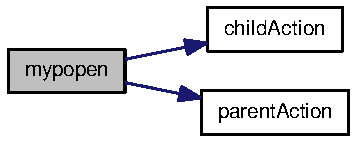
\includegraphics[width=104pt]{mypopen_8h_ac47876a41dddae340e5afa64489dec86_cgraph}
\end{center}
\end{figure}
\hypertarget{mypopen_8h_a1ee8542fc9a69bf1be706ed8c632ab69}{
\index{mypopen.h@{mypopen.h}!parentAction@{parentAction}}
\index{parentAction@{parentAction}!mypopen.h@{mypopen.h}}
\subsubsection[{parentAction}]{\setlength{\rightskip}{0pt plus 5cm}static FILE$\ast$ parentAction (int {\em fd}\mbox{[}2\mbox{]}, \/  int {\em unused\_\-end}, \/  int {\em used\_\-end}, \/  const char $\ast$ {\em type})\hspace{0.3cm}{\ttfamily  \mbox{[}static\mbox{]}}}}
\label{mypopen_8h_a1ee8542fc9a69bf1be706ed8c632ab69}

\printindex
\end{document}
